% Created 2021-12-12 Sun 20:17
% Intended LaTeX compiler: pdflatex
\documentclass[a4paper]{article}
\usepackage[utf8]{inputenc}
\usepackage[T1]{fontenc}
\usepackage{graphicx}
\usepackage{grffile}
\usepackage{longtable}
\usepackage{wrapfig}
\usepackage{rotating}
\usepackage[normalem]{ulem}
\usepackage{amsmath}
\usepackage{textcomp}
\usepackage{amssymb}
\usepackage{capt-of}
\usepackage{hyperref}
\documentclass{article}
\usepackage{here}
\usepackage{xcolor}
\usepackage{amsmath}
\usepackage{parskip}
\renewcommand\arraystretch{1.4}
\usepackage[margin=0.5in]{geometry}
\usepackage{minted}
\usepackage{multicol}
\definecolor{bg}{rgb}{0.95,0.95,0.95}
\newminted{java}{fontsize=\footnotesize,frame=single,framesep=2mm}
\newminted{text}{fontsize=\footnotesize,frame=single,framesep=2mm}
\author{Fatih Kaan Salgır - 171044009}
\date{}
\title{CSE443 - Object-Oriented Analysis \& Design - HW 3}
\hypersetup{
 pdfauthor={Fatih Kaan Salgır - 171044009},
 pdftitle={CSE443 - Object-Oriented Analysis \& Design - HW 3},
 pdfkeywords={},
 pdfsubject={},
 pdfcreator={Emacs 27.2 (Org mode 9.5)}, 
 pdflang={English}}
\begin{document}

\maketitle

\section*{Part 1}
\label{sec:orgac057b0}

The proxy pattern is used to provide safe access to data structure from multiple threads.
The synchronization problem is handled as in the readers-writers problem.
Synchronization is ensured using Java's \texttt{ReentrantReadWriteLock} by wrapping the methods of data structure with lock and unlock methods of the appropriate lock type.



\begin{figure}[htbp]
\centering
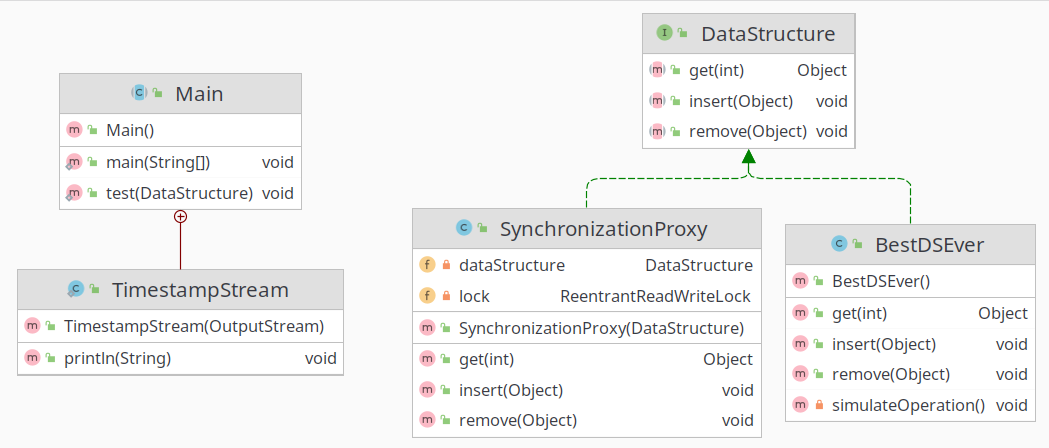
\includegraphics[width=.9\linewidth]{org-img/Part_1/2021-12-12_19-49-36_screenshot.png}
\caption{Class Diagram}
\end{figure}


To test, two threads are created in \texttt{Main} method, which calls \texttt{insert()}, \texttt{get()} and \texttt{remove()} respectively.
The output stream is modified to the print timestamp to demonstrate synchronization.
All operations are simulated using \texttt{Thread.sleep(1000)}.
So, the thread-unsafe version is expected to take about 3 seconds, and the thread-safe version is expected to take about 5 seconds (not 6 because both threads can read the data if no writers have the lock).


Output:

\begin{minted}[fontsize=\small,frame=single,framesep=3mm]{text}
[19:43:35.154400] ==== TEST: THREAD UNSAFE ====
[19:43:35.190006] Thread 1 started
[19:43:35.190242] Thread 2 started
[19:43:35.190334] inserting
[19:43:35.190360] inserting
[19:43:36.190616] getting
[19:43:36.190627] getting
[19:43:37.191169] removing
[19:43:37.191284] removing
[19:43:38.191698] Thread 1 finished
[19:43:38.191903] Thread 2 finished
[19:43:38.192742] ==== TEST: THREAD SAFE ====
[19:43:38.193765] Thread 1 started
[19:43:38.194064] Thread 2 started
[19:43:38.195885] inserting
[19:43:39.196609] inserting
[19:43:40.197320] getting
[19:43:40.197895] getting
[19:43:41.198459] removing
[19:43:42.199258] Thread 2 finished
[19:43:42.199355] removing
[19:43:43.200355] Thread 1 finished
\end{minted}


\newpage
\section*{Part 2}
\label{sec:org3b06d54}

Corresponding classes of composite design pattern;
\begin{itemize}
\item Component: \texttt{EmailComponent}
\item Composite: \texttt{EmailGroup}
\item Leaf: \texttt{Email}
\end{itemize}

\texttt{EmailComponent} is an abstract class instead of an interface because the email address field is common in both \texttt{Email} and \texttt{EmailGroup}.


\begin{figure}[htbp]
\centering
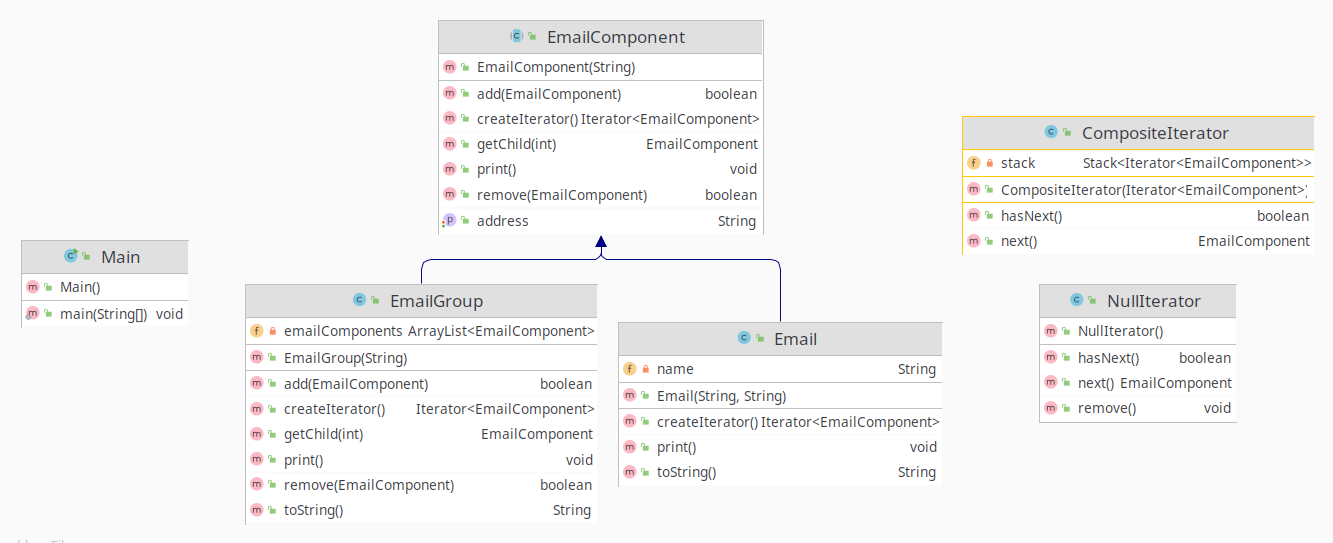
\includegraphics[width=.9\linewidth]{org-img/Part_2/2021-12-11_22-21-10_screenshot.png}
\caption{Class Diagram}
\end{figure}


Output:

\begin{minted}[fontsize=\small,frame=single,framesep=3mm,breaklines]{text}
==== TEST: print method called on an email =====
kendallroy@waystar.com Kendall Roy
==== TEST: print method called on an email group where elements are an email and an email group =====
loganroy@waystar.com Logan Roy
roysiblings@waystarroyco.com:{siobhanroy@waystar.com Siobhan Roy, kendallroy@waystar.com Kendall Roy, romanroy@waystar.com Roman Roy}
==== TEST: print method called on an email group where elements are emails and nested email groups =====
gerrikelman@waystar.com Gerri Kelman
tomwambsgans@waystar.com Tom
royfamily@waystarroyco.com:{loganroy@waystar.com Logan Roy, roysiblings@waystarroyco.com:{siobhanroy@waystar.com Siobhan Roy, kendallroy@waystar.com Kendall Roy, romanroy@waystar.com Roman Roy}}
\end{minted}
\end{document}
